\documentclass[conference]{IEEEtran}
\IEEEoverridecommandlockouts
% The preceding line is only needed to identify funding in the first footnote. If that is unneeded, please comment it out.
\usepackage{cite}
\usepackage{amsmath,amssymb,amsfonts}
\usepackage{algorithmic}
\usepackage{graphicx}
\usepackage{textcomp}
\usepackage{xcolor}
\def\BibTeX{{\rm B\kern-.05em{\sc i\kern-.025em b}\kern-.08em
    T\kern-.1667em\lower.7ex\hbox{E}\kern-.125emX}}
% This package makes the references clickable
\usepackage[colorlinks=true,citecolor=blue,linkcolor=blue,bookmarks=true]{hyperref}

% The code below allows you to write nice colourful comments
\usepackage{color,soul}

% Tikz
\usepackage{tikz}
\usetikzlibrary{positioning}

% Image placement
\usepackage{float}
\usepackage{caption}
\usepackage{subfig}

% Tables
\usepackage{graphicx}
% instead of \usepackage[table,xcdraw]{xcolor}
\usepackage{colortbl} 
\usepackage{lscape}

% Landscape


\begin{document}

\title{In-space mining and resource retrieval to Earth}

\author{\IEEEauthorblockN{Johnny Martin (Shaun) Lowis$^{a}$}
\IEEEauthorblockA{
\textit{$^{a}$Department of Mechanical Engineering, University of Canterbury, Christchurch, New Zealand} \\
jml190@uclive.ac.nz | 95700636 \\ ENME618 - Feasibility Study }
}

\maketitle

\begin{abstract}
The feasibility of an asteroid mining project, using a minimal viable 3U CubeSat was investigated. Key opportunities are rapidly evolving ride share technology and the Artemis program alongside government investing. Key threats are low raw value of collected material, with a best case of \$32.27 USD for 2kg retrieved mass, military involvement and uncertain legality. A review of current literature and analyses for the proposed system was included. Analysis on trends and future development indicates large potential in this sector.
\end{abstract}

\section{Introduction}
Humanity has seen exponential increases in energy and resource needs through the rapid technological evolution of the modern era: 1800 AD to now. The Kardashev scale \cite{1964SvA.....8..217K} is often used as an indicator of a civilisation's energy consumption, with humanity standing at Type 0.73 in 2023 \cite{Zhang2023}. As more complex and efficient technologies are developed, such as superconducting magnets, battery systems for electric vehicles and solar cells, the demand for higher quantities of materials grows. The amount of rare-Earth elements especially is of concern and a limiting factor in various industries, with concern geopolitically, due to their sourcing and processing being monopolised by China \cite{baskaran-2024}.

A proposed solution to these issues is the procurement of resources from space. In 2015, an asteroid containing an estimated \$5 trillion of platinum came within 6 lunar radiuses of Earth \cite{javelosa-2015}. Here a feasibility study is done on in-space mining of resources and their retrieval to Earth. To narrow the scope of this study, several methods to approach this problem is discussed, seen in Figure~\ref{fig:mining-circuits} and a specific method is chosen for evaluation. Only existing and near future technology (next 10 years) is considered.

\begin{figure}[H]
\centering
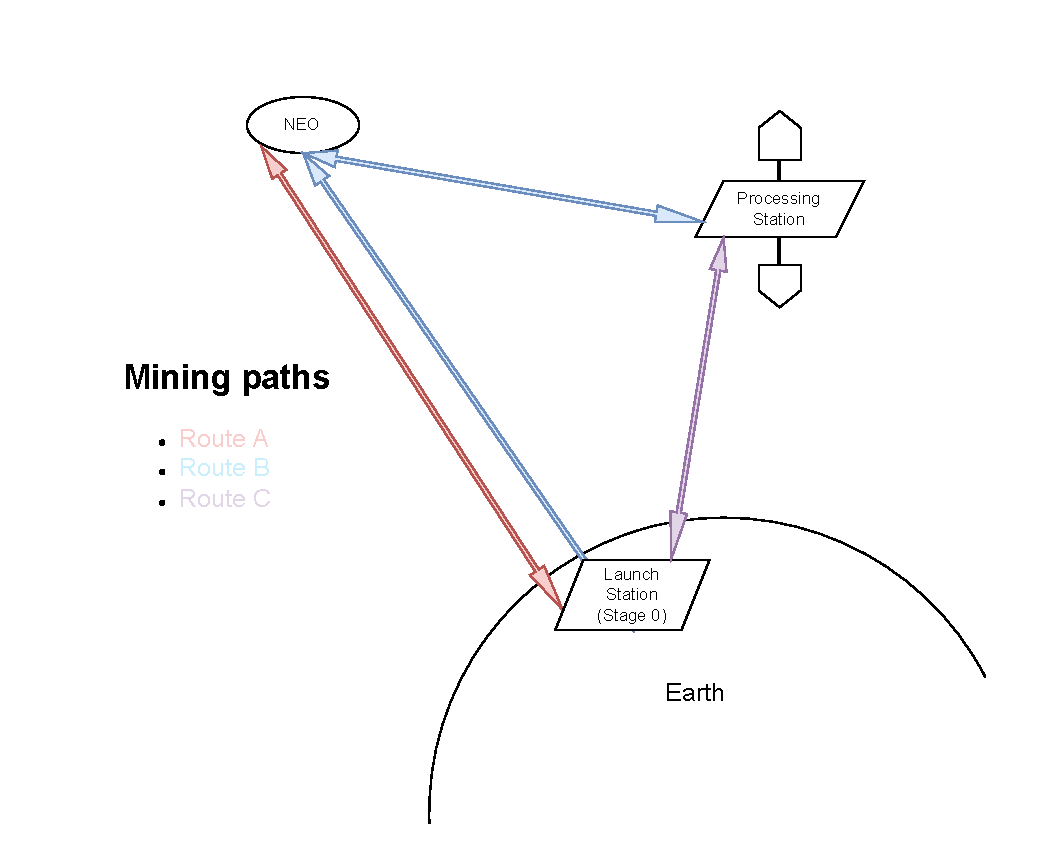
\includegraphics[width=.8\linewidth, height=5.5cm]{mining_paths.pdf}
\caption{\label{fig:mining-circuits}Possible mining circuits to Near Earth Object (NEO).}
\end{figure}

This study informs the reader on the feasibility of mining of asteroids. The process of in-space mining can be broken up into distinct phases shown in Figure~\ref{fig:mining-phases}. The red entries consist of these phases with some options shown to their right. The option chosen for this feasibility study is highlighted in blue. Further discussion on the choices are compared and contrasted throughout this study.

\begin{figure}[H] % 'H' makes sure the figure stays in place
    \centering
    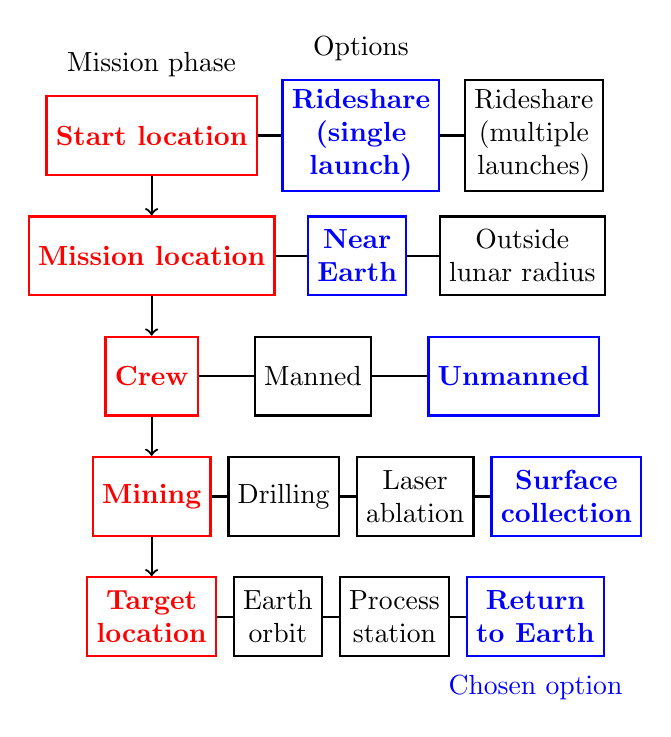
\begin{tikzpicture}[
      box/.style={rectangle, draw=red, thick, text=red, font=\bfseries, minimum width=1cm, minimum height=1cm},
      highlight/.style={rectangle, draw=blue, thick, text=blue, font=\bfseries, minimum width=1cm, minimum height=1cm},
      normal/.style={rectangle, draw=black, thick, minimum width=1cm, minimum height=1cm}
    ]
    
    % First column (bold red square boxes)
    \node[box] (start) {Start location};
    \node[highlight, right=.3cm of start, align=center] (rideshare1) {Rideshare \\ (single \\ launch)};
    \node[normal, right=.3cm of rideshare1, align=center] (rideshare2) {Rideshare \\ (multiple \\ launches)};
    
    % Second column (normal boxes, with highlighted one)
    \node[box, below=.5cm of start] (mission_location) {Mission location};
    \node[highlight, right=.4cm of mission_location, align=center] (near_earth) {Near \\ Earth};
    \node[normal, right=.4cm of near_earth, align=center] (outside_lunar) {Outside \\ lunar radius};
    
    % Third column (normal boxes, with highlighted one)
    \node[box, below=.5cm of mission_location] (crew) {Crew};
    \node[normal, right=.7cm of crew] (manned) {Manned};
    \node[highlight, right=.7cm of manned] (unmanned) {Unmanned};
    
    % Fourth column (normal boxes, with highlighted one)
    \node[box, below=.5cm of crew] (mining) {Mining};
    \node[normal, right=.2cm of mining] (drilling) {Drilling};
    \node[normal, right=.2cm of drilling, align=center] (laser_ablation) {Laser \\ ablation};
    \node[highlight, right=.2cm of laser_ablation, align=center] (surface_collection) {Surface \\ collection};
    
    % Fifth column (normal boxes, with highlighted one)
    \node[box, below=.5cm of mining, align=center] (target_location) {Target \\ location};
    \node[normal, right=.2cm of target_location, align=center] (earth_orbit) {Earth \\ orbit};
    \node[normal, right=.2cm of earth_orbit, align=center] (process_station) {Process \\ station};
    \node[highlight, right=.2cm of process_station, align=center] (return_earth) {Return \\ to Earth};
    
    % Arrows for the first column
    \draw[->, thick] (start) -- (mission_location);
    \draw[->, thick] (mission_location) -- (crew);
    \draw[->, thick] (crew) -- (mining);
    \draw[->, thick] (mining) -- (target_location);
    
    % First row:
    \draw[-, thick] (start) -- (rideshare1) -- (rideshare2);
    
    % Second row:
    \draw[-, thick] (mission_location) -- (near_earth) -- (outside_lunar);
    
    % Third row:
    \draw[-, thick] (mining) -- (drilling) -- (laser_ablation) -- (surface_collection);
    
    % Fourth row:
    \draw[-, thick] (crew) -- (manned) -- (unmanned);
    
    % Fifth row:
    \draw[-, thick] (target_location) -- (earth_orbit) -- (process_station) -- (return_earth);
    
    % Section headers:
    \node[above=0.1cm of start, text=black] {Mission phase};
    \node[above=0.1cm of rideshare1, text=black] {Options};
    
    \node[below=0.1cm of return_earth, text=blue] {Chosen option};
    
    \end{tikzpicture}
    \caption{Space mining phases and example options.}
    \label{fig:mining-phases}
\end{figure}

At the time of writing, the aerospace sector has entered an era of commonplace launching of the micro (10-100kg) to cubesat ($\le 1.33$ kg) sized satellites, though sizing is not standardised \cite{sat-sizing}. Rideshare companies such as Rocket Lab offer 1-2 microsats, 27 cubesats or some combination mounted to the fairing of their Electron rocket \cite{rocket-lab-usa-inc-2022} at a price of \$5 million USD. Cost per kg launched is the major limiting factor in space commercialisation. In this study a minimal viable space mining cycle along Route A in Figure~\ref{fig:mining-circuits}, is examined. An unmanned, surface collecting satellite with a re-entry mechanism, Figure~\ref{fig:mining-phases}, is examined, subject to the constraint of costing. This cost is compared with the returned resources obtained alongside a project plan, Environmental impact assessment and risk assessment, to estimate the validity of the industry.

\newpage
\section{Literature Review} \label{sec:lit-review}

First existing companies, with business models predicated on asteroid mining are examined. Current technology is compared and contrasted, from a cost-effectiveness view. The legal aspect of in-space ownership of resources as well as return to Earth is examined. Finally, areas of resource abundance are examined and an operating point is discussed for the mining activities.

\subsection{Existing industry}
In 2024, the space mining market size is estimated to be \$2 billion USD, with an annual growth rate of 19\% \cite{space-mining-insights}\cite{asteroid-mining-market}. Approaches to asteroid mining is in the developmental phase, with two main approaches to commercial viability: rapid iteration and multiple test deployments, or focus on proven R\&D for their technology stack. Some key players in this sector and an overview of their key strategy points are summarised in Table~\ref{tab:companies}.

% Please add the following required packages to your document preamble:
\begin{table}[H]
\centering
\resizebox{\columnwidth}{!}{%
\begin{tabular}{cccc}
\hline
\multicolumn{1}{|l|}{Company}                                                    & \multicolumn{1}{l|}{Headquarters}                          & \multicolumn{1}{l|}{\begin{tabular}[c]{@{}l@{}}Resource \\ target\end{tabular}} & \multicolumn{1}{l|}{\begin{tabular}[c]{@{}l@{}}Return\\ location\end{tabular}} \\ \hline
\textbf{Karman+}                                                                 & \begin{tabular}[c]{@{}c@{}}USA, \\ Colorado\end{tabular}   & Water                                                                           & \begin{tabular}[c]{@{}c@{}}Process\\ station\end{tabular}                      \\ \hline
\textbf{TransAstra}                                                              & \begin{tabular}[c]{@{}c@{}}USA, \\ California\end{tabular} & Biomasses                                                                       & \begin{tabular}[c]{@{}c@{}}Process\\ station\end{tabular}                      \\ \hline
\textbf{AstroForge}                                                              & \begin{tabular}[c]{@{}c@{}}USA,\\ California\end{tabular}  & Minerals                                                                        & \begin{tabular}[c]{@{}c@{}}Process\\ station\end{tabular}                      \\ \hline
\textbf{\begin{tabular}[c]{@{}c@{}}Asteroid\\ Mining\\ Corporation \\(AMC)\end{tabular}} & \begin{tabular}[c]{@{}c@{}}London,\\ England\end{tabular}  & \begin{tabular}[c]{@{}c@{}}Minerals,\\ water.\end{tabular}                      & Earth                                                                          \\ \hline
\end{tabular}%
}

\caption{Key companies and their mission plans \cite{steines-2023}.} \label{tab:companies}
\end{table}

Of the above companies, AstroForge follows the rapid iteration approach, with a successful test mission on April $15^{th}$, 2023 \cite{astroforge-update}. Karman+ is stil in the development phase, citing their future cost/kg at \$10,000 kg, with no real justification on this figure however \cite{karman-2024}. TransAstra is focusing on R\&D with a novel asteroid-capturing and optical mining approach \cite{transastra-2023}, targeting space debris removal as an objective. They also developed a telescope for asteroid surveying as their side-application. AMC has a terrestrially focused R\&D approach through the development of their SCAR-E robot, aiming for profitability through their robotics, before in-space operations \cite{amc-2024}. Key commonalities between these companies are \cite{scoles-2024}:

\begin{itemize}
    \item Side-ways applications, overlap with other industries during R\&D (except AstroForge).
    \item Multi-phase approach towards establishment.
    \item Based in, or co-governed by the USA geographically.
\end{itemize}

A difficult market to gain insight into is China. Their delegation submitted a resource declaration to the UN's Committee on the Peaceful Uses of Outer Space, outlining intent to utilize space resources \cite{jones-2024}, likely through China's Origin Space. In April 2021, they launched their NEO-1, a mining demonstrator and telescope \cite{cohen-2021}. Further updates since then have been lacking, though their monopolisation of rare-Earth minerals should mean a vested interest in this sector.

\subsection{In-space mining areas}\label{subsec:areas}
For NEO asteroids, very few have delta-v requirements under 4.5 km \cite{Elvis20111408} and identifying NEOs is difficult. Both due to their small viewing angle relative to Earth and interference from our atmosphere necessitating more effective observation in different spectral bands, ideally from outside Earth. though freely accessible via NASA JPL's Small-Body Database Query \cite{small-body-database-jpl} and LightCurve databases \cite{lightcurve-db}. The latter of which indicated 76 as water mining targets and 58 as potential platinum group targets \cite{Xie2023}. Unfortunately the downside of NEO's is having long synodic periods with Earth, when they are closest in orbit, which adds risk to missions as their next opportunity is on a large timescale.

\subsection{Current technology}\label{subsec:tech}
The critical enabling technology for space-mining are ride-share programs with commercial spaceflight companies Rocket Lab and SpaceX. This drastically lowered the cost barrier to entry to space. Consequently, to take advantage of these programs, industry needs to use systems small enough in size to remain cost effective, yet carry enough fuel for their missions.

The in-space fuel constraint is commonly referred to as the delta-v budget of the desired maneuver, given by the Tsiolkovskiy rocket equation \ref{eq:rocket-delta-v}\cite{tsiolkovskiy-1954}. This is between the orbit that the mining unit is delivered to by the ride-share rocket and the asteroid. 

\begin{equation}\label{eq:rocket-delta-v}
    \Delta v = v_e \ln{\frac{m_0}{m_f}} = I_{sp} g_0 \ln{\frac{m_0}{m_f}}
\end{equation}

Where:
\begin{align*}
    v_e = I_{sp} g_0 &= \text{is the effective exhaust velocity [m/s]} \\
    I_{sp} &= \text{specific impulse [s]} \\
    g_0 &= \text{standard gravity [m/s/s]} \\
    m_0, m_f &= \text{mass: initial, final [kg]}
\end{align*}

The mass available for propulsion is directly related to the distance the rocket can travel. Subject to this constraint, current industry focus on two avenues: fueling future space ventures by mining fuels such as water and biomasses, or searching for valuable near-Earth objects (NEO's). Both of these strategies benefit from lower delta-v needs. A NASA survey of small satellite propulsion systems \cite{parker-2016} indicated the need for further development of satellite propulsion systems. Miller et al \cite{Miller2021222} identified electric propulsion systems as the top performer for long duration small-sat missions, though these had delta v budgets half the size required for NEO missions. 

Further development of more advanced, efficient in terms of cost and mass budget propulsion systems are needed for the in-space access of asteroids to become more cost effective. Stack-able CubeSats of low U (2kg per U or cube) may be a good initial solution, as these are modular and can be configured for a specific mission and are commonly used for NEO missions \cite{aerospace4040058}.

For far future development, a delta-v map has been constructed of the Main Belt asteroids \cite{TAYLOR201873}, between Mars and Jupiter which show promise, with delta-v requirements frequently under 4km. This may be more accessible once NASA's Artemis program yields a launch base from the Moon's south pole. Human landing on the moon was aimed at 2024 when the program was announced in 2020, however it is currently scheduled for 2026, though these goals are subject to much debate. As such further investigation beyond NEO is omitted.

\subsection{Law and governance}\label{subsec:law}
The legality of asteroid mining is still in its infancy. In the US, Shaw \cite{shaw2013asteroids} applied the general mining law as incentive to asteroid mining, leading to a bill introduced in 2014. This resulted in the ASTEROIDS Act \cite{TRONCHETTI2014193} and the passing of the Commercial Space Launch Competitiveness Act that grants US citizens the right to claim resources from space. This was met with controversy on the international stage from other countries, particularly China and Russia. The Artemis Accords have attempted to alleviate these concerns, with 35 countries having signed agreeing to access rights to resources over their "safety cone" projected from the Moon, though the Commercial Space Launch Competitiveness Act has not been repealed. 

The UN has a Committee on the Peaceful Uses of Outer Space, who convened in April, 2024. Sessions from April $16-18^{th}$ \cite{united-nations-no-date} focused on the US's FCC moving to regulate orbital debris, mandating end of life de-orbits. Special consent and a license is also required for radio frequency bands used by satellites. The session by Henry Hertzfeld urged the need for uniform legal liability for in-space actions. These were presented on Thursday, 18 April 2024. Further presentations focused on fair and distributed access to space resources. However property rights and mining laws are very much a grey area at the time of writing, with no further clear regulation on licensing, zoning or liability established.

A survey of 27 countries by Hornsey et. al \cite{su14074119} suggested "that mining companies have a “social license to operate” for mining asteroids, but less so for lunar mining." This indicates an overall positive stance towards in-space mining of resources for NEO's.

\section{Method}\label{sec:method}
From Section~\ref{sec:lit-review}, we conclude that for profitability and least cost a project that is:

\begin{enumerate}
    \item Based in the USA (for legal reasons, discussed in Section \ref{subsec:law}).
    \item Uses a SpaceX or RocketLab rideshare (due to cost).
    \item Targets NEO asteroids (due to current propulsion limits and no existing in-space processing or refueling infrastructure, Section \ref{subsec:areas})
    \item Follows the CubeSat design (for simplicity, modularity and Rideshare fairing support as in Section \ref{subsec:tech})
\end{enumerate}

Will be recommended and used for further analysis.

\textit{1. US facilities:}
Facilities in the USA are required to adhere to the Environmental Protection Agency's regulations \cite{epa-2024}. Aerospace activities also fall under the Department of Defence, hence International Traffic in Arms Regulations (ITAR) apply. This restricts the hiring of individuals to US persons. While this adds barriers to hiring and potentially increased salary expenses, the benefit is the legal right to claim resources from space.

At a minimum, the facilities should have two clean rooms: these are required as Foreign Object Debris (FOD) is highly dangerous to aerospace components with small orifices and can lead to faulty propulsion systems and leaks. FOD is likely a cause for two NASA astronauts being stranded on the ISS until early 2025, due to 5 failures with Boeing's Starliner's 28 thrusters \cite{rnz-news-2024}. A clean room for processing incoming goods such as commercial off the self (COTS) parts and a clean room for assembly is standard practise. Machinery needed should include at least a single 6-axis CNC machine for in-house manufacturing of needed parts, which often have highly complex geometries. An additive manufacturing facility is also useful, but can be outsourced. Other than this, various machines like helium leak detectors and vibration tables can either be sourced for in-house use, or externally contracted. The assumption here is that contracting these requirements is readily available, in terms of timelines and costing.

\textit{2. Ride-share:}
To utilise a ride-share, the system must adhere to the requirements outlined by the provider. As the market setter, SpaceX generally stipulates these requirements. Among them are requirements on total system leak rate (tested with Helium as this is a very small and inexpensive gas), maximum vibration tolerance and mechanical coupling to the fairing. The assumption is that engineers employed for the project can cost, source and execute the necessary operations, while adhering to these requirements. They are often evolving and are copyrighted and released at the discretion of SpaceX. \cite{rocket-lab-usa-inc-2022}. It is assumed that a mission is available at the time of the project and costs \$300,000 USD \cite{spacex-rideshare-cost-2025}.

\textit{3. NEO target:}
Using the LightCurve asteroid database \cite{lightcurve-db} is the most cost effective targeting solution. An alternative is developing sensing instrumentation such as telescopes, as is done by TransAstra \cite{transastra-2023}. The benefit of this approach is that more reachable NEO asteroids may be discovered, but the risk is that there is no payoff for this additional launch if this is not the case. The assumption here is a that one of the 58 platinum NEO asteroids are reachable within the timeline of this project.

\textit{4. Satellite design:}
A simple approach is to follow the CubeSat design. These are composed of a number of 10x10x10 [cm] Units (U's), where a good size for this project is a 3U satellite. These can be bought off the shelf, for example from NanoAvionics \cite{nanoavionics-2023}, in Figure~\ref{fig:nano-av-3U}. This has the benefit of offloading the in-house design process of much of the satellite. It comes with power management systems via its solar panels and battery pack and radio communication as well as an on-board computer. 

\begin{figure}[H]
\centering
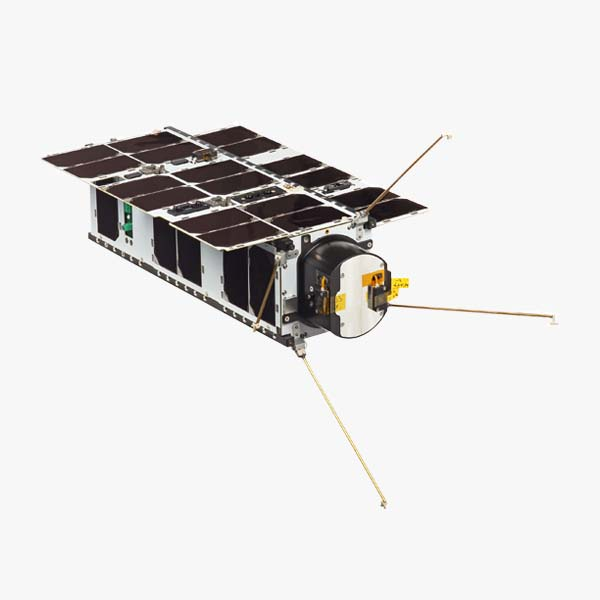
\includegraphics[width=\linewidth]{nano-av-3U.jpg}
\caption{\label{fig:nano-av-3U}NanoAvionics' 3U nanosatellite bus M3P, retrieved Sept 11, 2024 \cite{nanoavionics-2023}}
\end{figure}

The mission payload is up to 3kg and size up to 2U. The assumption here is that the demonstration vehicle for the mining project is capable of collecting a sample from the surface of the asteroid and contain enough propellant to return to a de-orbit maneuver to return the sample to Earth. Specific propulsion systems are subject to mission requirements \cite{zakirov-2001} and is an evolving market.

Development and design of the collection system is therefore to be done as part of the project and will form the bulk of the project's timeline and basis of costing. The mission will follow Route A, in Figure~\ref{fig:mining-circuits}. It is assumed that the propellant needed is factored into the design and conforms to the mass budget of this satellite bus.

An intensive body of work is needed for on-orbit operations, which will determine the mission plan. This informs the cost and duration of the engineering design needed. As part of on-orbit operations, the decomissioning process is planned. The satellite should have some payload bay that can survive re-entry, for example designed out of Titanium should be used. This must adhere to  IADC Space Debris Mitigation Guidelines (2007): “If a spacecraft or orbital stage is to be disposed of by re-entry into the atmosphere, debris that survives to reach the surface of the Earth should not pose an undue risk to people or property.” 

The U.S. Government Orbital Debris Mitigation Standard Practices stipulates: “If a space structure is to be disposed of by reentry into the Earth’s atmosphere, the risk of human casualty will be less than 1 in 10,000.” \cite{jet-propulsion-laboratory-2018}. The assumption is that an appropriate plan is to be constructed by engineers with the technical capability to adhere to these requirements. For logistics, retrieval is assumed to be done over uninhabited land for ease of access, with a mechanism that prevents the loss of the asteroid sample.

\section{Results}
Analysis related to the feasibility of asteroid mining are carried out. Key assumptions and overviews are provided in this section, with further discussion carried out in Section~\ref{sec:discussion}.

\subsection{Project planning}\label{sec:project}

\begin{figure}[H]
\centering
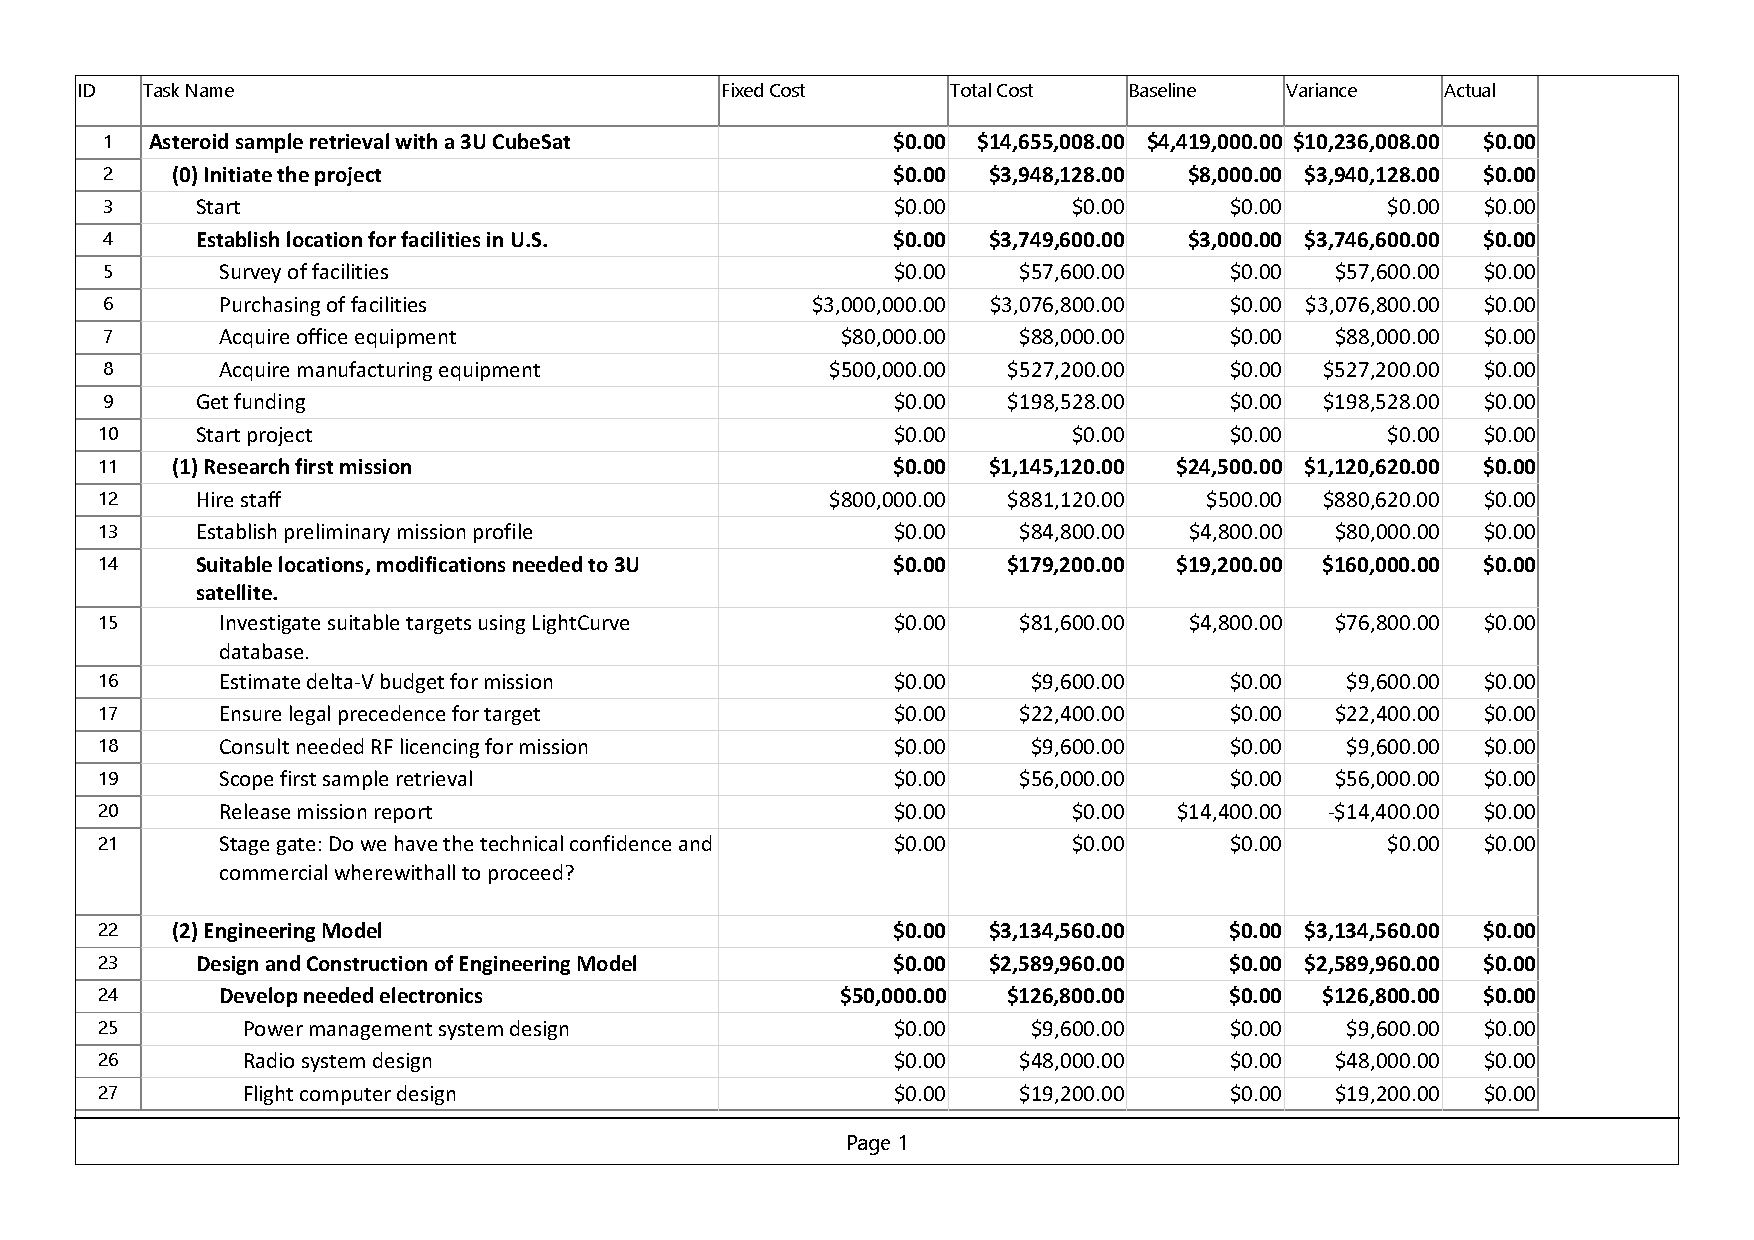
\includegraphics[page=1, width=\linewidth]{project_inital.pdf}
\includegraphics[page=2, width=\linewidth]{project_inital.pdf}
\includegraphics[page=3, width=\linewidth]{project_inital.pdf}
\caption{\label{fig:proj}Project plan, using Microsoft Project Professional.}
\end{figure}

A project plan has been outlined in MS Project. Simplifying assumptions were made and added to the notes section of the respective tasks. This is accessible in the attached \verb|jml190_enme618_feasibility.mpp| file. It was assumed that most testing, design and iteration would need minimal iteration. Another simplifying assumption was a very small team size. For greater accuracy and more efficient time planning, projects, especially assigned to the Systems Engineer resource should be broken up into sub-tasks for members of a team. Due to the technical complexity and rapid evolution of technology relevant to this project, it was assumed that further specificity around task management for systems smaller than sub-systems would be too subject to change by the time they are reached. 

As such, an overview approach was taken to construct this project plan. The key points here are attention given to costs and balancing work loads for resources. The overall plan follows the sub-sections as described in Section~\ref{sec:method}. For costing, it was assumed that the project would use an Engineering Model of the mining system, then a Flight Model. The latter would be at least as expensive as the prior, with additional changes from learning made post test campaign of the EM. The process of selling the collected sample is considered outside the scope of the project and some estimates for this is covered in the financial analysis section.

\subsection{Environmental effects: Life cycle analysis}

The life cycle of asteroid mining is unique as future technology may enable an open loop to resourcing for this cycle. Indicated in Figure~\ref{fig:lca} by the red triangle, this may result in unprecedented sustainability, as previously defined by conservation of resources on Earth. Currently however, various risks and ecological concerns are inherent to the components used for asteroid mining systems.

\begin{figure}[H]
\centering
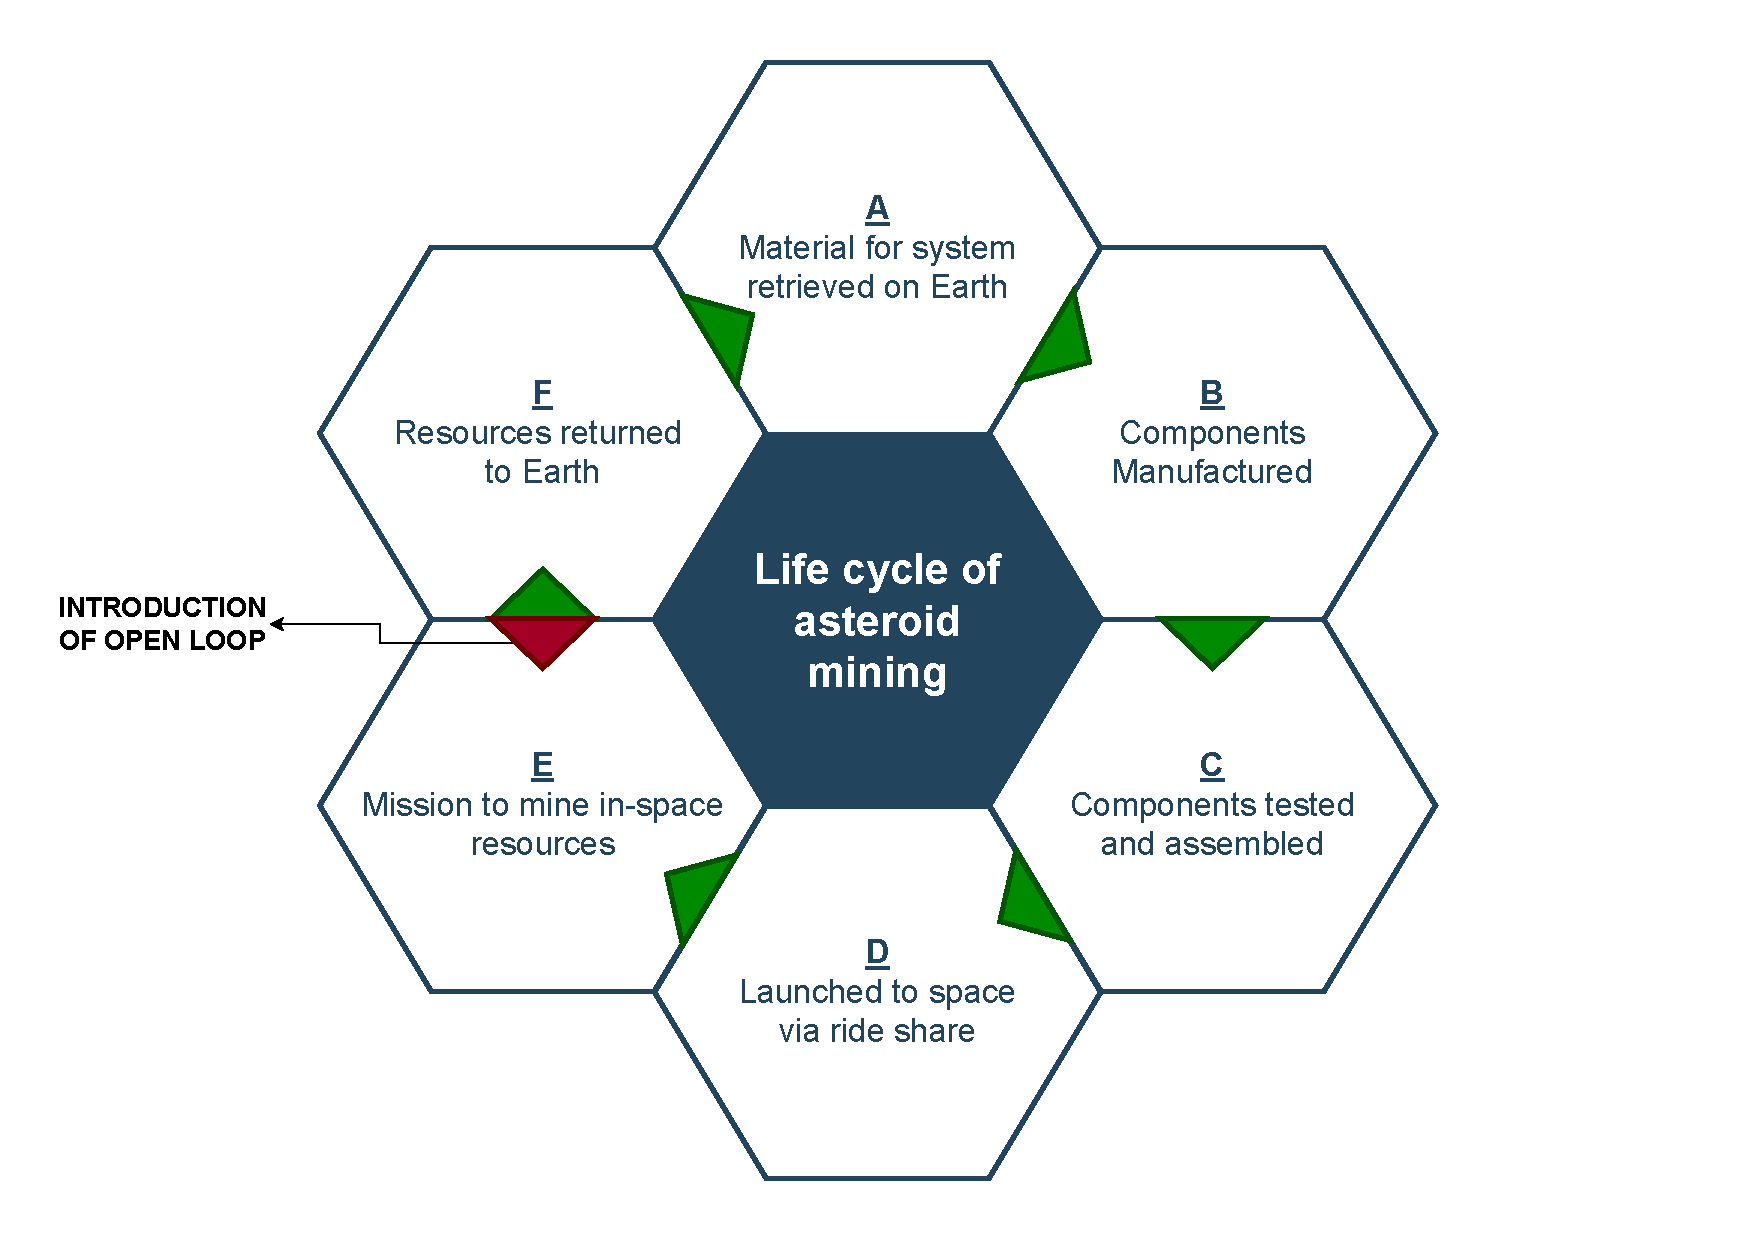
\includegraphics[width=\linewidth]{lca.pdf}
\caption{\label{fig:lca}Life cycle of the outlined project, with annotation on where future progress may enter the cycle.}
\end{figure}

The assumptions and limits made for the phases in Figure~\ref{fig:lca} are:
\begin{itemize}
    \item[A] Wherever possible, it is assumed that the supplier of materials needed ensured due diligence with respect to sustainability.
    \item[B] It is assumed that best practices with respect to environmental consideration and ecological preservation was followed for the manufacturing process.
    \item[C] Minimisation of harmful chemical or other waste products and proper disposal of these are assumed.
    \item[D] A re-usable ride share company is to be used for this section.
    \item[E] An asteroid is selected that prioritises human safety and minimises risk of debris negatively impacting human life or the ecosystem.
    \item[F] Where needed, atmospheric burn-up is designed to encompass complete combustion to minimise waste.
    
\end{itemize}

All of these are further discussed later in this report. These assumptions are used to provide better axes of comparison for the scenarios used below.

Two key variables are investigated for scenarios on the life cycle of the project are in-space refueling and increased regulation or liability to mining operators. These change the de-orbiting of the system at the end of its mission and change the scope of the analysis to encompass in-space liability, respectively. These have been broken down into baseline (no change), favourable and unfavourable cases for each of these two changes.

\subsubsection{Baseline}
Current technology is maintained for the duration of the project. As in-space operations in general has not significantly changed since the Apollo era, this is a likely course of technological evolution for at least the next 10 years. In this case, resources would be returned to Earth alongside the mining system being burned up upon re-entry. The legal landscape of American dominance persists, with no additional liability added. 

\subsubsection{Favourable change; in-space refueling}
In-space depots that can provide propellant to systems in-orbit opens up two main economic avenues: procurement of fuel from asteroids, such as water ice. The other avenue is repeat missions with larger return payloads. Construction of vehicles for mining in-space may also be possible in this case, completely de-coupling the Life Cycle. From an environmental point of view, sourcing resources from space may entail little to no human or ecological suffering, if done in a carefully planned and sustainable manner.

\subsubsection{Unfavourable change; in-space refueling}
An unfavourable change in this sector would be the advent of in-space refueling, but it is highly monopolised and exploitative of the in-space environment. This may lead to severely depleted resources in and around Earth as well as too much space junk being produced from these resources, resulting in further environmental destruction.

\subsubsection{Favourable change; legal}
An environmentally favourable change in the legal realm is greater liability that private operators face. Historically, unregulated enterprise has lead to severe habitat depletion and exploitation of natural resources. It would be beneficial to both undiscovered environments and to future generations of humankind to approach in-space mining in a sustainable and environmentally conscious way. The main way that this has been achieved in the past is by making corporations or individuals subject and liable for their actions.

\subsubsection{Unfavourable change; legal}
Following on from the favourable change, the environmentally unfavourable change would be less regulation and liability for in-space actions. This may lead to international warfare and crimes committed with no clear authoritative body. Human conflict leads to habitat and environmental destruction, alongside the human suffering. A worst-case scenario is if conflict or exploitation of the in-space environment leads to adverse effects for life on Earth. Debris fields from waste or conflict may lead to loss of vital satellite internet and GPS technologies. Factors that change Earth's albedo affect the amount of solar radiation that reaches the surface, thereby harming ecosystems through a causal chain.

\subsection{Risk assessment}
We examine key threats and opportunities for the project. The horizon is viewed as beyond just the scope of this project, but also focuses on in-space asteroid mining as a whole. Aspects specific to this project are discussed further in Section~\ref{sec:discussion}.

For scoring, we apply the rubric in Figure~\ref{fig:risk-score} for Table~\ref{tab:pestle}.

Further discussion of the risk matrix is continued in Section~\ref{sec:discussion}, though the two most valuable opportunities are:

\begin{itemize}
    \item Novelty of space retrieved resources (300)
    \item Higher than expected resource quality, deconstructing monopolies on resources (both 200)
\end{itemize}

The two most costly threats are:

\begin{itemize}
    \item Operation causes military tensions (-500)
    \item Weaponisation of space resources (-500)
\end{itemize}

Where the current socio-political and socio-economic volatility of this emerging market is evident.

\begin{figure}[H]
\centering
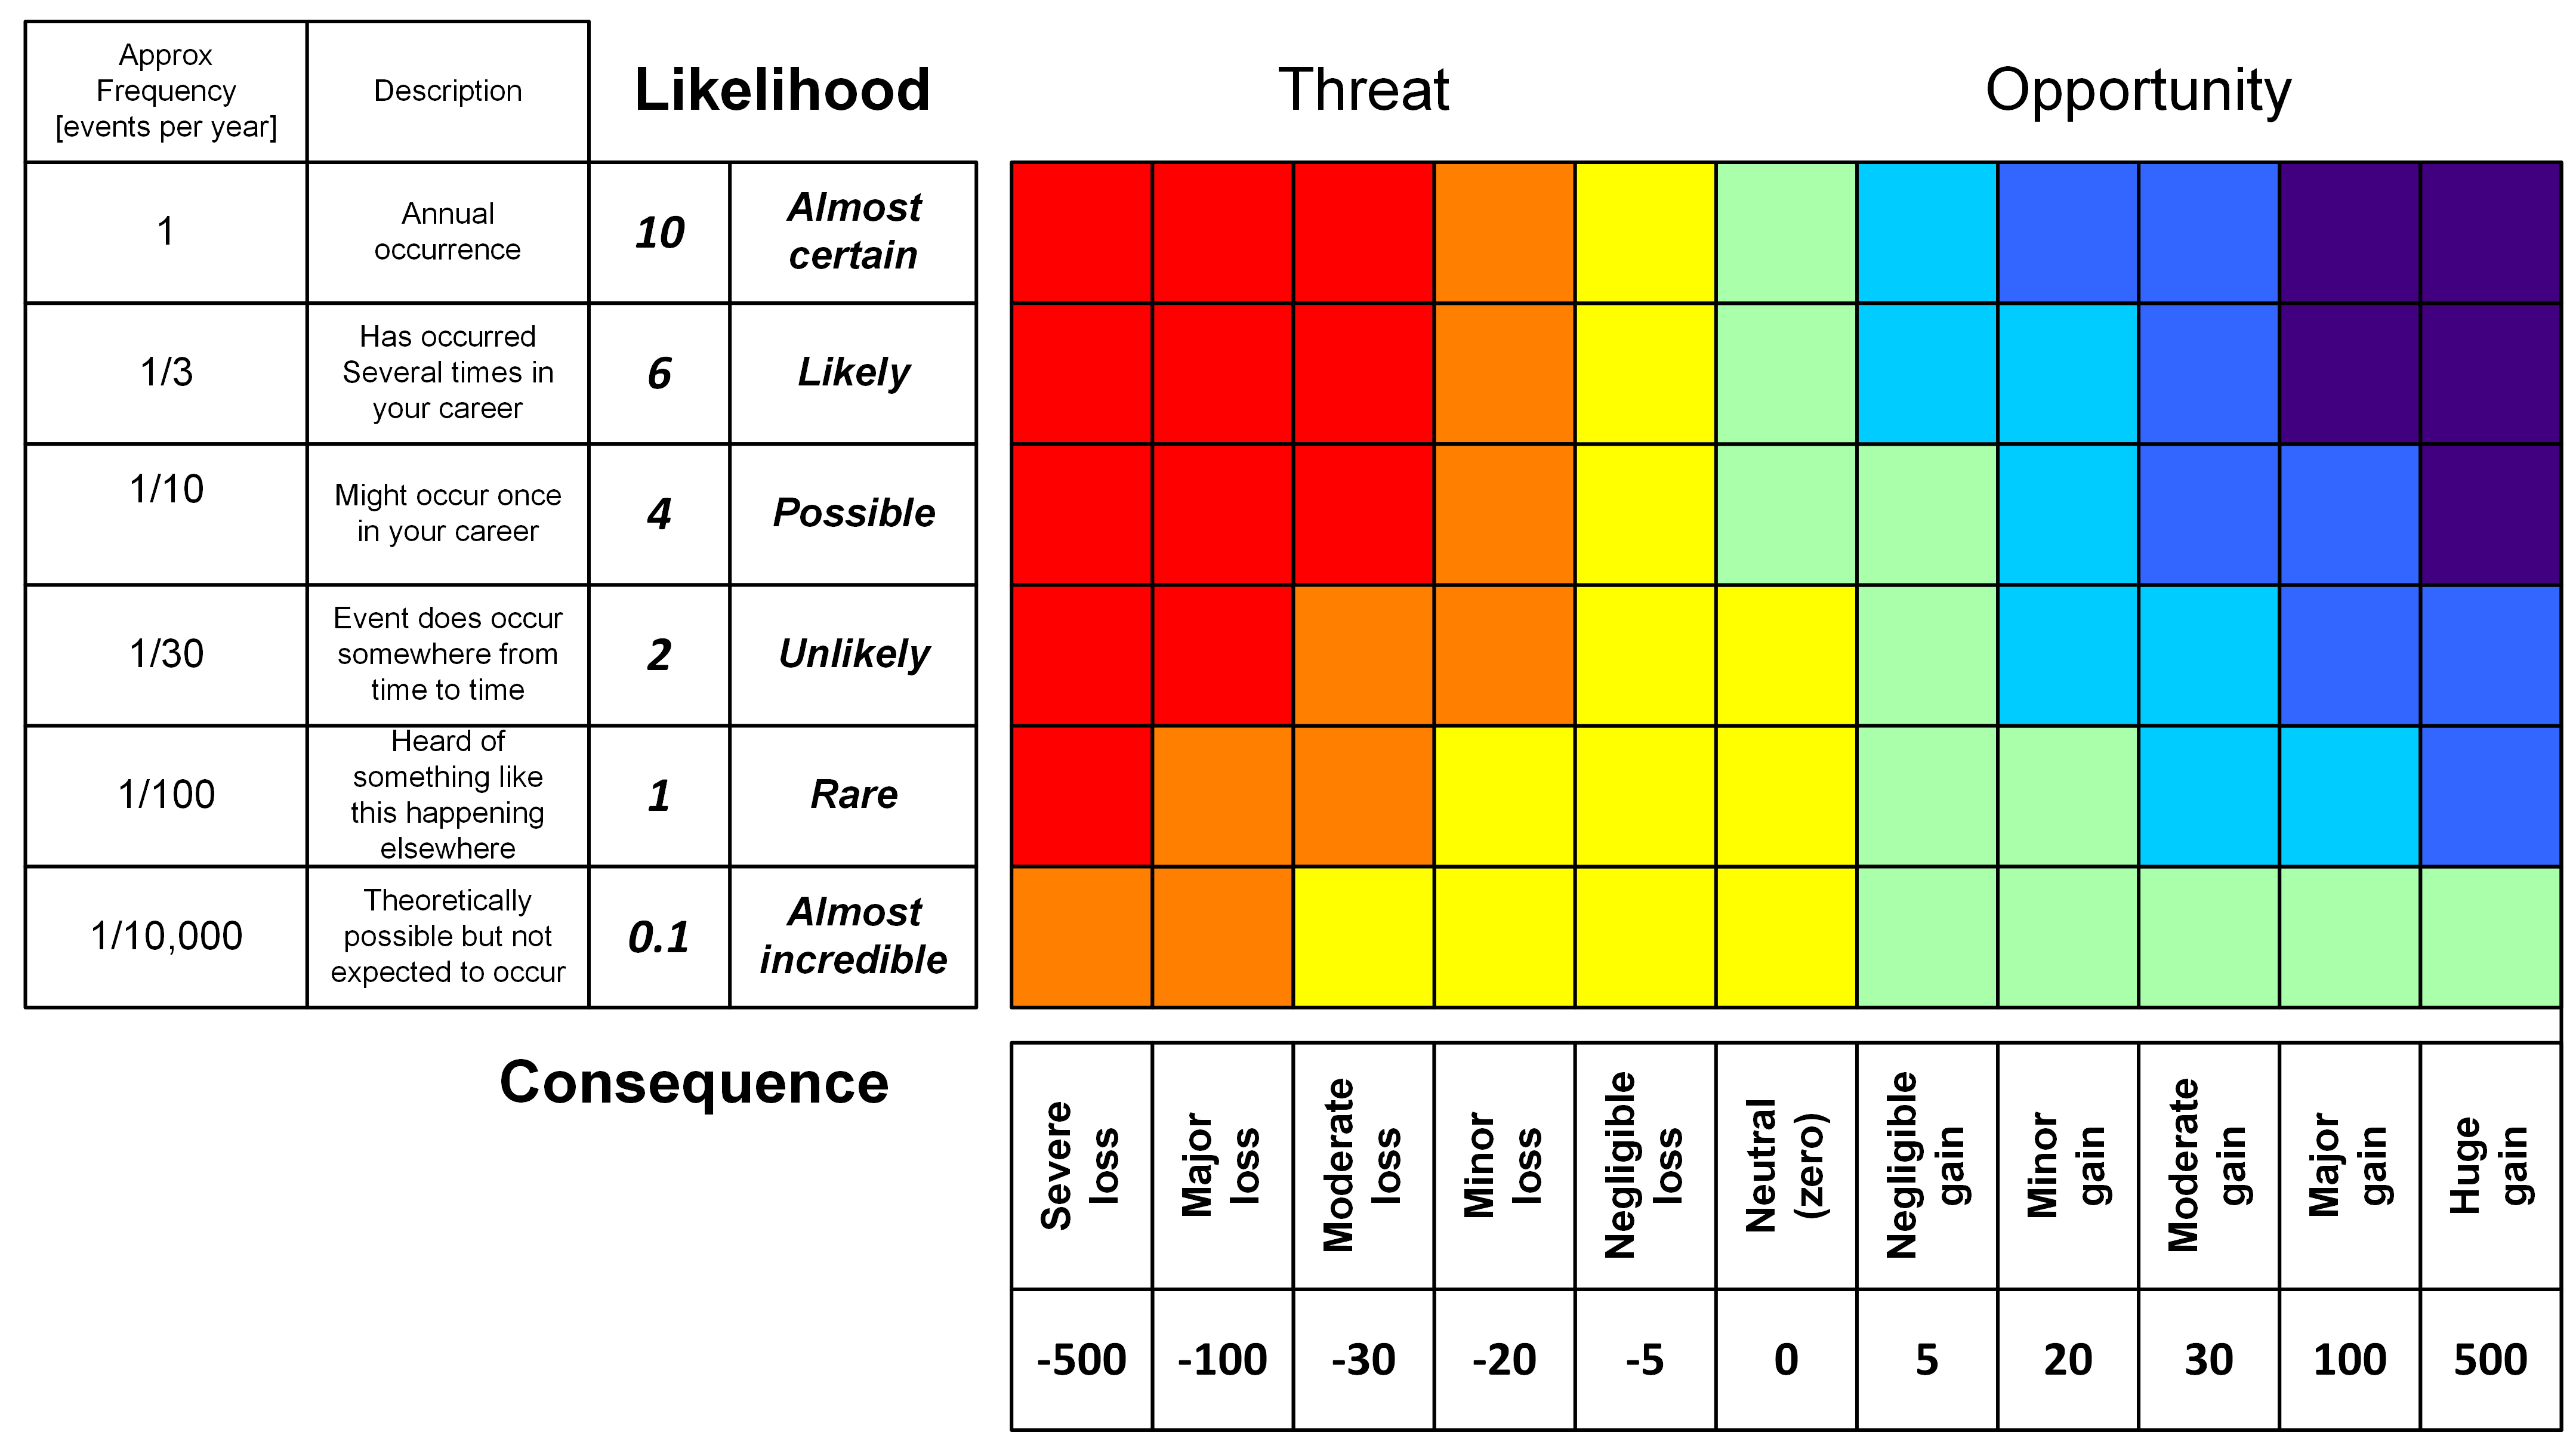
\includegraphics[width=\linewidth]{risk_map_scoring.png}
\caption{\label{fig:risk-score}Scoring criteria for risk assessment, as provided by Dirk Pons, New Zealand\cite{risk-scoring-template}.}
\end{figure}

\begin{table}[H]
\centering
\resizebox{\columnwidth}{!}{%
\begin{tabular}{|l|l|l|l|}
\hline
\rowcolor[HTML]{C0C0C0} 
\cellcolor[HTML]{343434} & Political                                                                                                    & Economical                                                                                         & Societal                                                                                             \\ \hline
I. Threat                & \begin{tabular}[c]{@{}l@{}}Operation causes\\ military tensions.\end{tabular}                                & \begin{tabular}[c]{@{}l@{}}Pay-off of mining is \\ not worth the cost.\end{tabular}                & \begin{tabular}[c]{@{}l@{}}Public view on \\ asteroid mining \\ worsens.\end{tabular}                \\ \hline
\rowcolor[HTML]{FFCE93} 
Likelihood               & Rare, 1                                                                                                      & Possible, 4                                                                                        & Rare, 1                                                                                              \\ \hline
\rowcolor[HTML]{FFCCC9} 
Consequence              & Severe loss, -500                                                                                            & Moderate loss, -30                                                                                 & Negligible loss, -5                                                                                  \\ \hline
\rowcolor[HTML]{CBCEFB} 
Risk score               & -500                                                                                                         & -120                                                                                               & -5                                                                                                   \\ \hline
II. Threat               & \begin{tabular}[c]{@{}l@{}}Other countries \\ dispute resources.\end{tabular}                                & \begin{tabular}[c]{@{}l@{}}Market instability \\ from over-supply.\end{tabular}                    & \begin{tabular}[c]{@{}l@{}}Public view on \\ in-space operations \\ worsens.\end{tabular}            \\ \hline
\rowcolor[HTML]{FFCE93} 
Likelihood               & Unlikely, 2                                                                                                  & Possible, 4                                                                                        & Rare, 1                                                                                              \\ \hline
\rowcolor[HTML]{FFCCC9} 
Consequence              & Moderate loss, -30                                                                                           & Major loss, -100                                                                                   & Negligible loss, -5                                                                                  \\ \hline
\rowcolor[HTML]{CBCEFB} 
Risk score               & -60                                                                                                          & -400                                                                                               & -5                                                                                                   \\ \hline
III. Threat              & \begin{tabular}[c]{@{}l@{}}Operation is used as\\ justification for \\ negative political acts.\end{tabular} & \begin{tabular}[c]{@{}l@{}}Fines from other \\ countries, due to \\ mission location.\end{tabular} & \begin{tabular}[c]{@{}l@{}}Public view on \\ space exploration\\ worsens.\end{tabular}               \\ \hline
\rowcolor[HTML]{FFCE93} 
Likelihood               & Possible, 4                                                                                                  & Almost incredible, 0.1                                                                             & Rare, 1                                                                                              \\ \hline
\rowcolor[HTML]{FFCCC9} 
Consequence              & Major loss, -100                                                                                             & Severe loss, -500                                                                                  & Negligible loss, -5                                                                                  \\ \hline
\rowcolor[HTML]{CBCEFB} 
Risk score               & -400                                                                                                         & -50                                                                                                & -5                                                                                                   \\ \hline
IV. Opportunity          & \begin{tabular}[c]{@{}l@{}}Deconstructing \\ monopolies on resources.\end{tabular}                           & \begin{tabular}[c]{@{}l@{}}Novelty of space\\ retrieved resources.\end{tabular}                    & \begin{tabular}[c]{@{}l@{}}Positive views \\ encourage \\ public investment.\end{tabular}            \\ \hline
\rowcolor[HTML]{FFCE93} 
Likelihood               & Unlikely, 2                                                                                                  & Almost certain, 10                                                                                 & Possible, 4                                                                                          \\ \hline
\rowcolor[HTML]{9AFF99} 
Consequence              & Major gain, 100                                                                                              & Moderate gain, 30                                                                                  & Minor gain, 20                                                                                       \\ \hline
\rowcolor[HTML]{CBCEFB} 
Risk score               & 200                                                                                                          & 300                                                                                                & 80                                                                                                   \\ \hline
V. Opportunity           & Unifying space efforts.                                                                                      & \begin{tabular}[c]{@{}l@{}}Higher than expected \\ resource quality.\end{tabular}                  & \begin{tabular}[c]{@{}l@{}}Positive views \\ allow new \\ marketing and \\ advertising.\end{tabular} \\ \hline
\rowcolor[HTML]{FFCE93} 
Likelihood               & Rare, 1                                                                                                      & Unlikely, 2                                                                                        & Possible, 4                                                                                          \\ \hline
\rowcolor[HTML]{9AFF99} 
Consequence              & Moderate gain, 20                                                                                            & Major gain, 100                                                                                    & Minor gain, 20                                                                                       \\ \hline
\rowcolor[HTML]{CBCEFB} 
Risk score               & 20                                                                                                           & 200                                                                                                & 80                                                                                                   \\ \hline
\rowcolor[HTML]{C0C0C0} 
\cellcolor[HTML]{343434} & Technological                                                                                                & Legal                                                                                              & Environmental                                                                                        \\ \hline
I. Threat                & \begin{tabular}[c]{@{}l@{}}Weaponisation \\ of space resources.\end{tabular}                                 & \begin{tabular}[c]{@{}l@{}}Restriction on \\ areas of mining.\end{tabular}                         & \begin{tabular}[c]{@{}l@{}}Debris generated \\ from activities.\end{tabular}                         \\ \hline
\rowcolor[HTML]{FFCE93} 
Likelihood               & Almost incredible, 0.1                                                                                       & Possible, 4                                                                                        & Possible, 4                                                                                          \\ \hline
\rowcolor[HTML]{FFCCC9} 
Consequence              & Severe loss, -500                                                                                            & Negligible loss, -5                                                                                & Moderate loss, -30                                                                                   \\ \hline
\rowcolor[HTML]{CBCEFB} 
Risk score               & -50                                                                                                          & -20                                                                                                & -120                                                                                                 \\ \hline
II. Threat               & \begin{tabular}[c]{@{}l@{}}Defense contracting\\ for space resource \\ claims.\end{tabular}                  & \begin{tabular}[c]{@{}l@{}}Increased liability \\ for actions.\end{tabular}                        & \begin{tabular}[c]{@{}l@{}}Unforeseen \\ asteroid impacts.\end{tabular}                              \\ \hline
\rowcolor[HTML]{FFCE93} 
Likelihood               & Possible, 4                                                                                                  & Rare, 1                                                                                            & Almost incredible, 0.1                                                                               \\ \hline
\rowcolor[HTML]{FFCCC9} 
Consequence              & Major loss, -100                                                                                             & Moderate loss, -30                                                                                 & Severe loss, -500                                                                                    \\ \hline
\rowcolor[HTML]{CBCEFB} 
Risk score               & -400                                                                                                         & -30                                                                                                & -50                                                                                                  \\ \hline
III. Threat              & \begin{tabular}[c]{@{}l@{}}Superior \\ competing \\ technology.\end{tabular}                                 & Ceasure of operations.                                                                             & \begin{tabular}[c]{@{}l@{}}Unforeseen \\ solar activity.\end{tabular}                                \\ \hline
\rowcolor[HTML]{FFCE93} 
Likelihood               & Possible, 4                                                                                                  & Rare, 1                                                                                            & Unlikely, 2                                                                                          \\ \hline
\rowcolor[HTML]{FFCCC9} 
Consequence              & Minor loss, -20                                                                                              & Severe loss, -500                                                                                  & Moderate loss, -30                                                                                   \\ \hline
\rowcolor[HTML]{CBCEFB} 
Risk score               & -80                                                                                                          & -500                                                                                               & -60                                                                                                  \\ \hline
IV. Opportunity          & \begin{tabular}[c]{@{}l@{}}Cost reduction \\ from new \\ technology.\end{tabular}                            & Supportive legislation.                                                                            & \begin{tabular}[c]{@{}l@{}}Unexpected\\ resource \\ abundance.\end{tabular}                          \\ \hline
\rowcolor[HTML]{FFCE93} 
Likelihood               & Unlikely, 2                                                                                                  & Rare, 1                                                                                            & Almost incredible, 0.1                                                                               \\ \hline
\rowcolor[HTML]{9AFF99} 
Consequence              & Minor gain, 20                                                                                               & Moderate gain, 30                                                                                  & Huge gain, 500                                                                                       \\ \hline
\rowcolor[HTML]{CBCEFB} 
Risk score               & 40                                                                                                           & 30                                                                                                 & 50                                                                                                   \\ \hline
V. Opportunity           & \begin{tabular}[c]{@{}l@{}}Enabling further \\ mining areas \\ from new \\ technology.\end{tabular}          & \begin{tabular}[c]{@{}l@{}}Precedence as \\ an early player.\end{tabular}                          & \begin{tabular}[c]{@{}l@{}}Unexplored \\ areas.\end{tabular}                                         \\ \hline
\rowcolor[HTML]{FFCE93} 
Likelihood               & Unlikely, 2                                                                                                  & Possible, 4                                                                                        & Likely, 6                                                                                            \\ \hline
\rowcolor[HTML]{9AFF99} 
Consequence              & Moderate gain, 30                                                                                            & Moderate gain, 30                                                                                  & Minor gain, 20                                                                                       \\ \hline
\rowcolor[HTML]{CBCEFB} 
Risk score               & 60                                                                                                           & 120                                                                                                & 120                                                                                                  \\ \hline
\end{tabular}%
}
\caption{A risk matrix of threats and opportunities alongside their likelihood and consequences. Rows are denoted by colour, vertically continued for legibility.}
\label{tab:pestle}
\end{table}

\subsection{Human factors}
The key risks to human life are when the system is in the assembly stage on Earth, where the risk moves to a financial nature once the system is assembled. The most dangerous sub system on the mining satellite are the pressure vessels and by extension the propulsion system. Depending on the type of propulsion, the system may not be feasible to hot-fire test at all. For example, hydrazine is a commonly used propellant as it is a mono propellant, typically using Iridium as a catalyst. It is also highly  dangerous to human health. The EPA classifies it as a Group B2 human carcinogen and it is also highly corrosive and reactive.


\begin{figure}[H]
\centering
\includegraphics[page=2, angle=90, width=\linewidth]{bowtie.pdf}
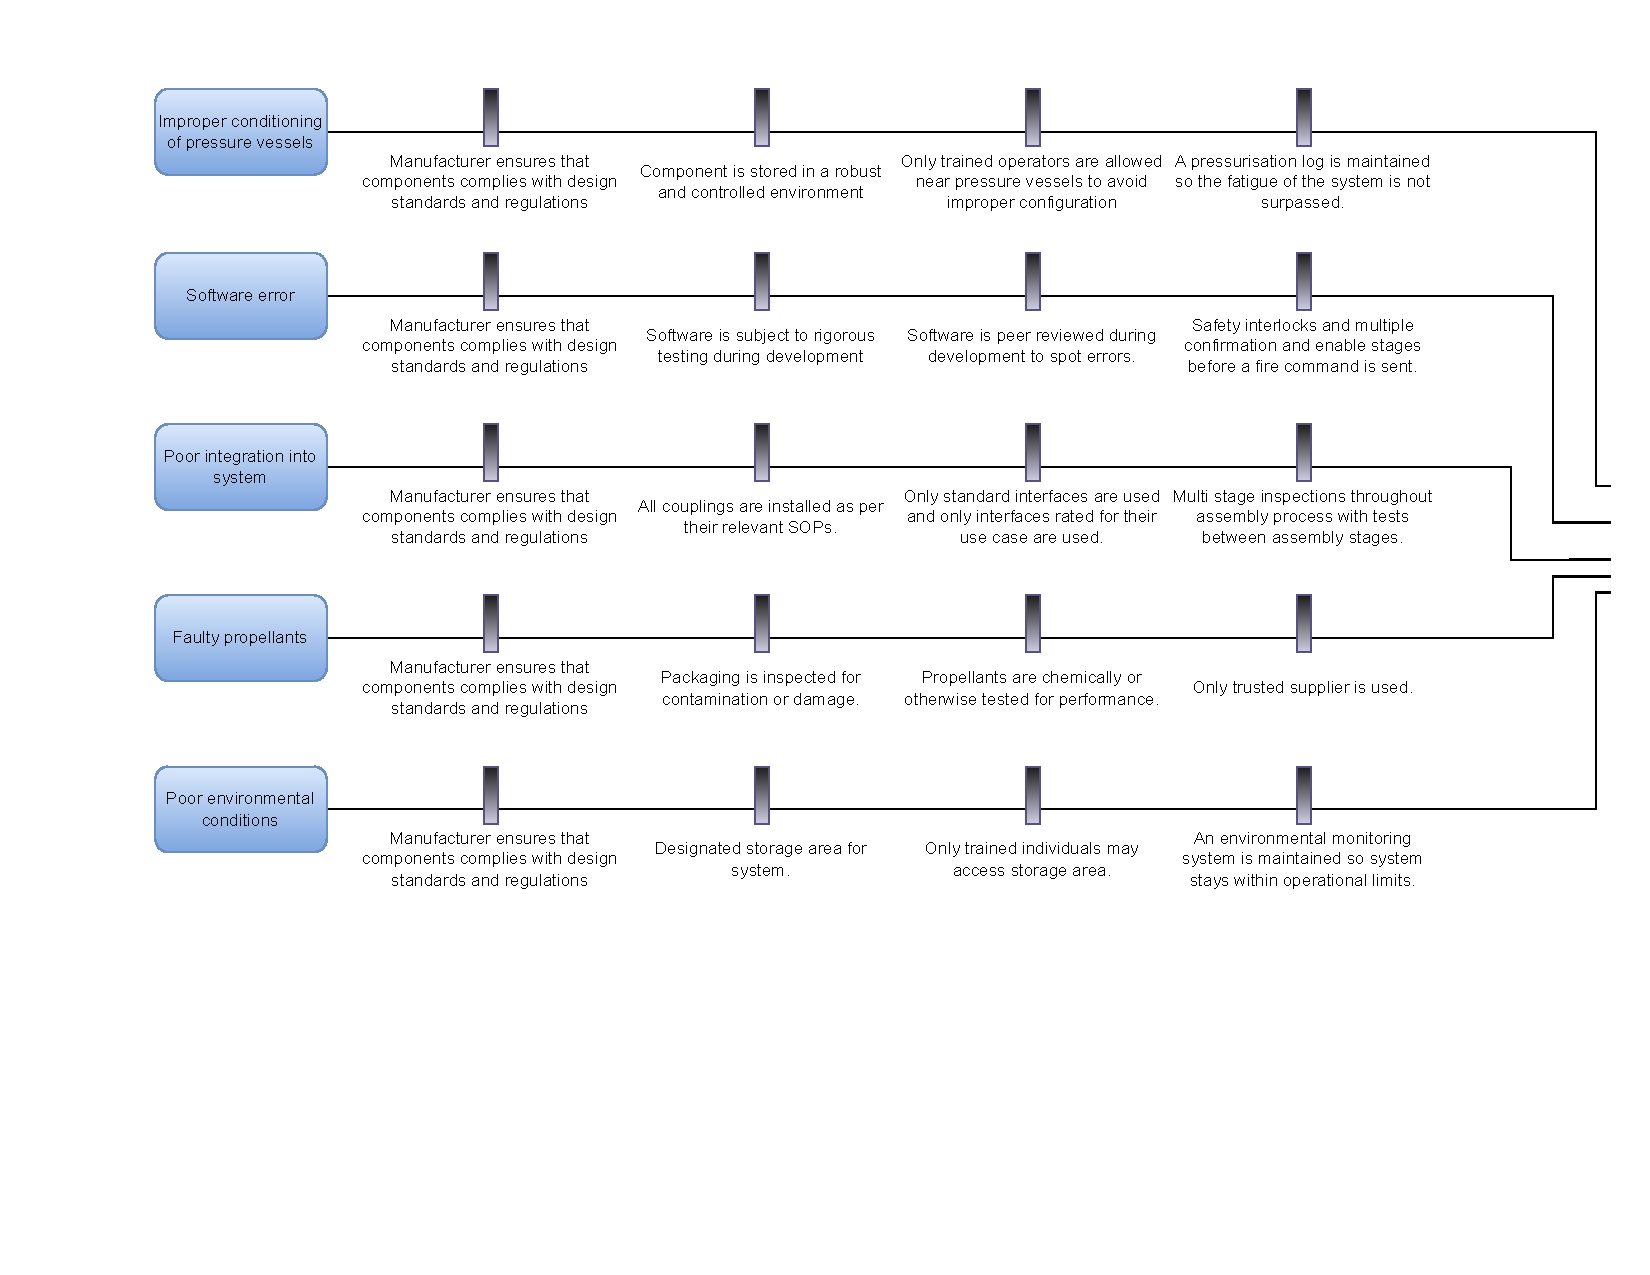
\includegraphics[page=1, angle=90, width=\linewidth]{bowtie.pdf}

\caption{\label{fig:bowtie}Bowtie analysis on a misfire or detonation of the propulsion system. File also submitted as \textit{bowtie.pdf}.}
\end{figure}

\subsection{Life cost analysis}
Using the costing outlined in the project plan, we construct a cash flow analysis. This project will have no pay-offs until the payload itself is recovered. The only direct monetary gain, other than funding, of this project will be in the form of selling collected resources. Conservatively, this project is estimated to cost \$6-10,000,000 USD, depending on constructing an Engineering Model or only constructing a Flight Model with very conservative labour costs. This was chosen to be a minimal viable costing basis, informing the reader of funding and costing needed.

\begin{figure}[H]
\centering
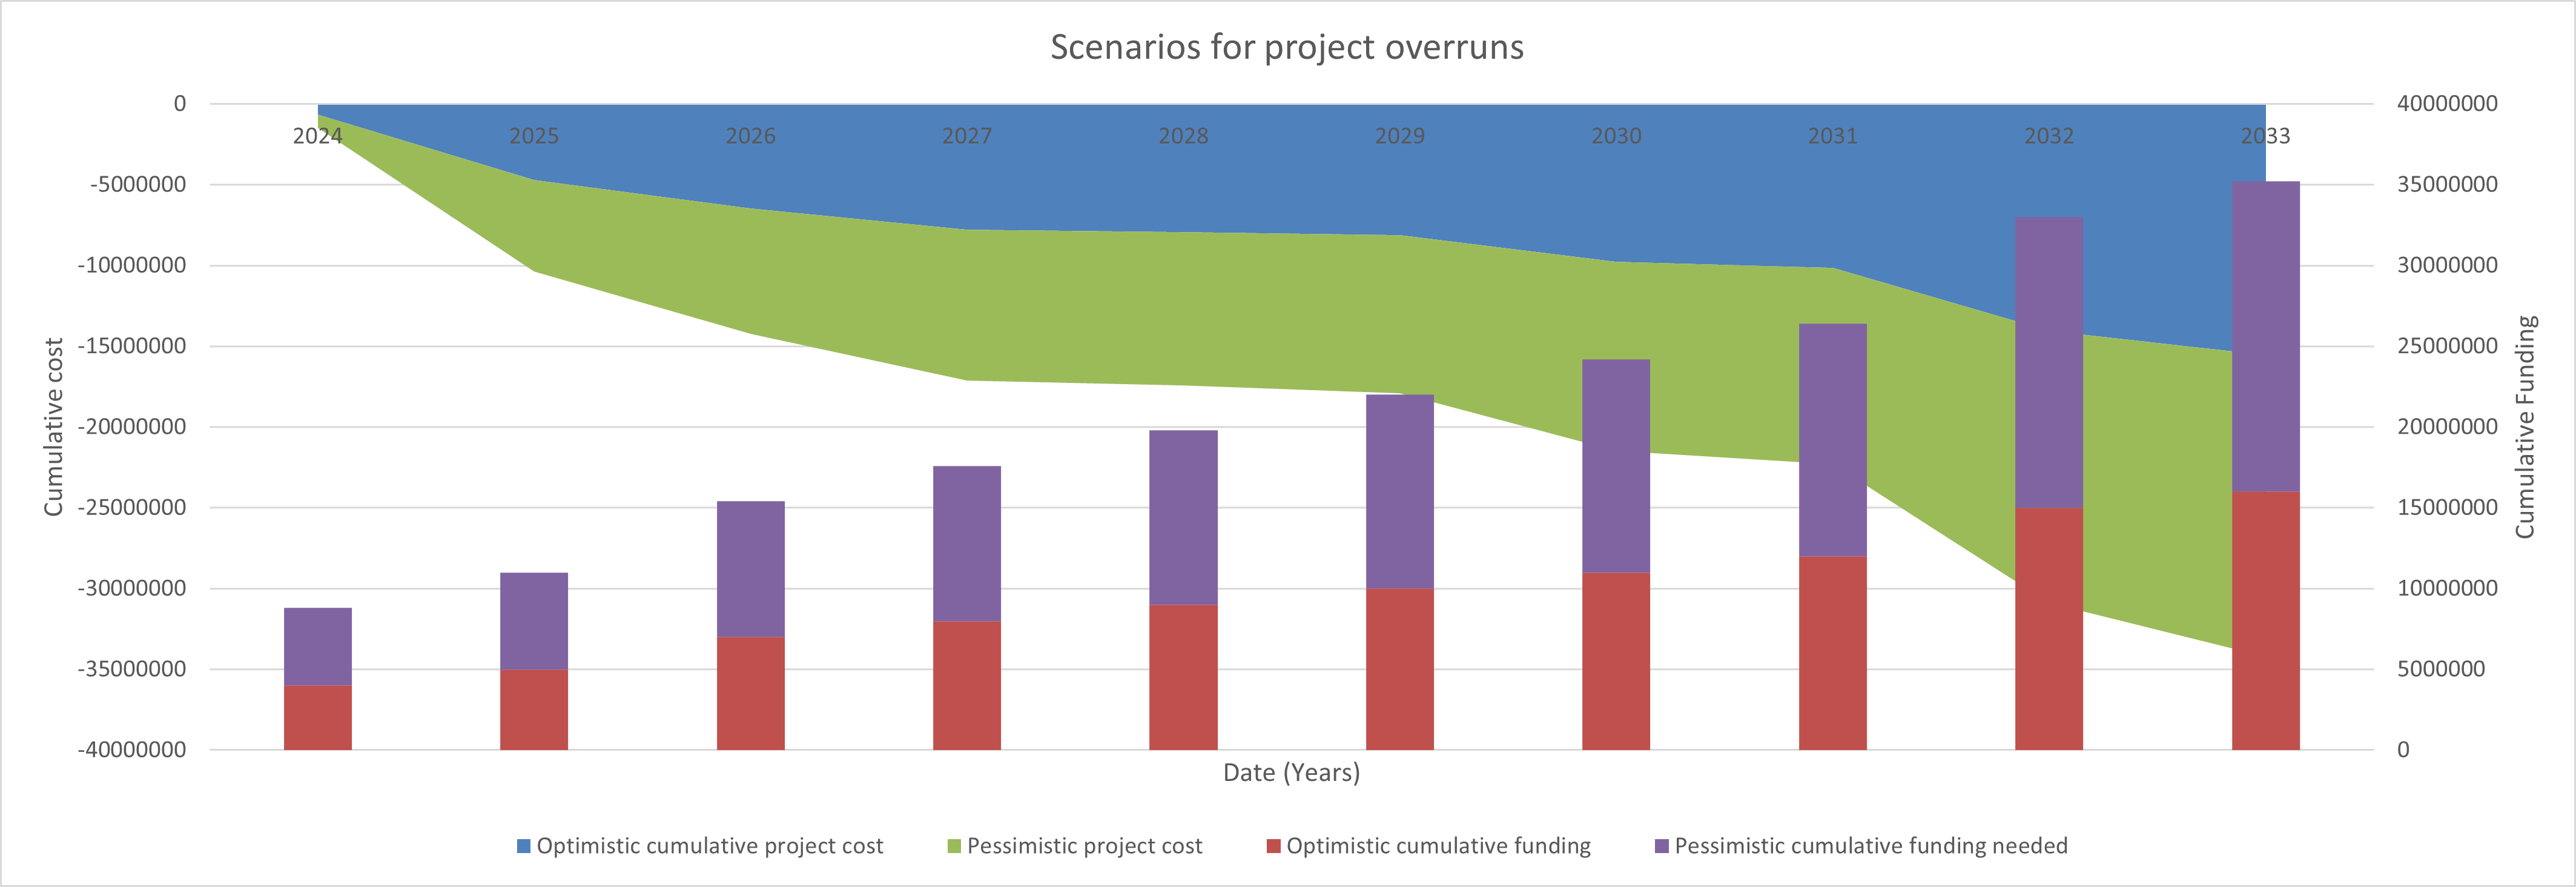
\includegraphics[width=\linewidth]{cash_flow_projection.png}
\caption{\label{fig:cashflow}Optimistic and pessimistic costing and funding for a minimal asteroid mining project.}
\end{figure}

The reader should view the financial aspect of this project as a technology demonstrator. A method of garnering investor interest and sentiment, with future-looking prospects, as that is where all the income will be from. The payload bay of this CubeSat can only accommodate 3kg, where a conservative mass budget for a retrieval mechanism would be at least 1kg. Assuming an asteroid containing platinum is targeted as earlier discussed, a best case return of a surface collection mission may yield some platinum. On Earth, platinum is mined at a yield of 3-6 grams per tonne of ore. The platinum content of an asteroid is most recently estimated to be between $\approx 6$ to 230ppm (or grams per tonne), (K. M. Cannon, et. al 2023 \cite{CANNON2023105608}).  Assuming 2kg of asteroid material is collected,  which at the best case means 0.00046g of platinum being returned, yields \$0.0148 USD. At the current price per g of platinum of \$32.27 USD. Hence a cash flow analysis of selling mined goods is not insightful.

As such, variance in costing was examined in Figure~\ref{fig:cashflow}, where the optimistic scenario is no cost overruns and a pessimistic scenario included 20\% cost overruns. This approach was taken because the costing perspective used in the project plan was conservative. Therefore it is very highly unlikely that the project may under-run in costs.

This financial analysis assumed no income from sources other than funding for the duration of the project. A more accurate valuation may be found by including estimates for grants from government and private bodies. These will have large effects on the viability of this project and is not unrealistic. Recently, the first ever private space walk was achieved as part of SpaceX's Polaris Dawn mission campaign by billionaire Jared Isaacman \cite{comerford-2024}, who also funded the campaign. As such a mission with some direct financial repayment (from novelty of asteroid mined material) could be expected to be funded by investors entirely. AstroForge recently raised \$40 million USD \cite{foust-2024}, as a current example.

\subsection{Societal effects}
As outlined in Section~\ref{subsec:law}, there is a sound basis for companies' "social license to operate" to utilise in-space resources. The key areas of uncertainty are the effects on the global socio-economic supply chain if this technology becomes widespread. If larger quantities of a mineral or resource is retrieved than has ever been mined on Earth, it is speculative at best as to how this would affect existing markets. 

Countries that are less developed are commonly the source of raw natural resources, especially rare minerals such as gold and platinum. These countries have historically been subject to much exploitation during colonialism due to this mineral wealth. The affect of sudden resource abundance at a global scale has a low chance of being positive on these countries, as their resources are a key economic foundation for trade.

More developed countries are less susceptible to the negative aspect of an increase in supply in natural resources as these countries generally export goods that require more processing steps, further down the global supply chain. As such the immediate effects of these changes are more likely to be positive than negative for developed countries. They are also generally more capable of space programs, which require high levels of education, infrastructure and international relations to be successful. As such, developed countries should find entry into this sector much easier than developing countries.

A worst-case outcome for the sudden overabundance of natural resources would be further privatisation and siloing of economic resources by private companies. A best-case outcome would be large improvements in technology and engineering, enabled by more resource availability and lower cost of construction and manufacturing. This leads to more rapid prototyping and development of both production and R\&D activities.

\subsection{Other analyses}
As the in-space mining field is a new and innovative sector, it can be difficult to objectively assess the value and risks that lie therein. A useful framework to provide insight into such cases is using VIRO. To aid with applying this framework, we define:

\begin{itemize}
    \item Near-term: Next 5 years, good insights based on current trends.
    \item Medium-term: Next 10-15 years, broader ideas should remain applicable from current trends.
    \item Long-term: Over 20 years from now, speculative.
\end{itemize}

We apply these in the case that asteroid mining as a venture in general is successful and unsuccessful. Unsuccessful sections are more prompt as they lead to termination in that aspect of the venture, not because the positive sections are more favoured by the author.

\textbf{Valuable}
Assuming success, the near-term value proposition of asteroid mining is initially in novelty and as part of the current resurgence of public interest in space operations. The medium-term depends mostly on the outcomes of the Artemis program and the status of the Moon as a refueling station for further operations. The long-term value lies in the Main Belt asteroids, between Mars and Jupiter.

Assuming failure, the near term value is negative, with costs far exceeding funding. This persists into the future, unless technological advances take place in the medium to long term.

\textbf{Inimitable}
Assuming success, we can broadly say that compared to Earth-sourced minerals, space-sourced minerals are distinct and inherently inimitable. In the near-term, genuineness of space as the source of asteroid mined material is assured as less than a handful of missions are expected to be carried out. In the medium term, it may be necessary to establish some certification as to the source of the material as these become more introduced to supply chains. In the long term, ideally space-sourced resources are the norm, though this does not remove from its distinctiveness.

Assuming failure, it may be that space-sourced materials are impossible to distinguish from Earth-sourced materials, leading to difficulty in the medium to long term in proving the origins of said materials.

\textbf{Rare}
Assuming success, near term rarity of asteroid mined resources would be extremely high, with auctions and platforms of sale focused on the novelty being the primary method of trade. In the medium term, rarity decreases with number of missions. In the long term, for a thriving industry, space-sourced material and minerals should be far more commonplace than Earth-sourced materials.

Assuming failure, space-sourced minerals and resources may remain a rarity for the foreseeable future, as few missions to retrieve them are successful.

\textbf{Organisation}
Assuming success, near term more funding and competing players in the market emerge, encouraging a growing competitive industry. In the medium term, industry may shift to in-space processing and refueling for further development of the sector. In the long term, human occupation of areas of space increasingly far from Earth may develop as a result of resource abundance, furthering the industry's development.

Assuming failure, a large private sector effort may be needed in the future, such as SpaceX, in that they lowered the barriers to entry to the commercial aspects of space. This changed decades of technological stagnation, following the Apollo missions. This may be required for a capable large organisation that could provide a meaningful impact in this sector.

\section{Discussion/Conclusion}\label{sec:discussion}
The author declares their intent to remain objective and unbiased. While the author acknowledges that inherent bias cannot be overcome, they hereby aim to minimise their personal stance and reflect objectively on their professional recommendation. \\

The project outlined in Section~\ref{sec:project} was constructed for a minimal 3U CubeSat. For high risk missions, such as ones to outer space where the system is unreachable after assembly and deployment, it is common to first build an Engineering Model, then a Flight Model. This is a also a common aerospace practise. The assumption on this project was the inclusion of this approach, as well as cost minimisation. For example, hiring human resources and including these as a resource was done if the same resource were to be re-used multiple times, such as a GNC Expert. A general trend with aerospace companies is keeping resourcing in-house as much as possible, so this project plan aimed to reflect that with budget for in-house tooling and manufacturing. The costing was generally conservative, with flat fixed cost estimates alongside the cost of labour for relevant employees. This is to reflect the uncertainty of cost in a growing and variable industry. Key factors here that the reader should consider are distance and difficulties for procurement from suppliers (such as import taxes and insurance) and more accurate sub-task timelines. Timelines were generally very simplified, with high-demand resources such as the system and software engineers being allocated several balanced tasks. The reader would benefit from adding their own team compositions and costs to this project. It should be considered a template for a minimal cost system that should be able to conduct a demonstration mission. 

The timelines for the mission act as placeholders. These would vary massively subject to more information and requirements for the mission itself. For example, the Hayabusa2 asteroid sampling mission surveyed the asteroid 162173 Ryugu for a year and a half. The reader should modify the commissioning section to their own mission. \\

A large assumption has been made around hardware, software and electronics functionality outside geostationary orbit. As one moves further from Earth's magnetic field, the shielding effects of the field diminish. As such, radiation primarily from the Sun, but also from cosmic sources is far stronger. This results in wearing of materials as ionised particles from the Sun impact the surface of the system, as well as decreased lifetimes of electronics and bit flip errors in software. The latter occurs when ionising radiation delivers enough energy to either add electrons, or adjust their position in electronics. All of these components can be designed around, with radiation hardened equipment, but would massively increase the cost of the project. Radiation hardened components is also a specialty product, usually made to order, hence costing information is difficult to estimate. The reader is encouraged to consult with suppliers directly about this. The author reached out to NanoAvionics about the functionality of their 3U CubeSat and its pricing for a mining mission and was advised it would not be possible to use their system, likely for the above reasons. See Appendix Section~\ref{apdx:email}. \\

The above assumption has direct ties to the proposed life cycle of the system. It may be that the introduction of the open loop in Figure~\ref{fig:lca} may never occur, as some replacement components may always need to be manufactured on Earth. This could be due to in-space conditions having adverse effects on manufacturing, for example, the placing of electronics components and the common approach of using re-flow soldering for large quantities of products may not work at all in space. However, the introduction of an additional in-space manufacturing or production cycle would still be a large cost reduction, as these components won't need to be launched with a rocket as part of their cost. A key to the establishment of industry is transport. Without in-space refueling, the cost of movement in space is too large due to a constrained fuel budget for missions to enable replacement of components. As such, the favourable change of in-space refueling may be a key enabling factor for asteroid mining. This is because mining requires large distances to be covered and the cost would be reduced by orders of magnitude if parts could be replace in-orbit. The latter won't be cost effective until the fuel budget for moving to replacement or maintenance stations is high enough. \\

The risk assessment outlined sources of largest concern and opportunity for the project. The military aspect and concern may seem unwarranted, however recent establishment of the United States Space Force and China's People's Liberation Army Aerospace Force show concerning trends in the militarisation of space. The reader should be aware of the developments in this sector and proceed with caution. Military involvement with aerospace projects is hardly unexpected. The key opportunities of the venture are around its novelty and the current lack of information of the in-space mining environment where the largest value lie. This was further reflected in the VIRO analysis, where the near-term value of the industry is from novelty. The financial gain, as shown via a cash flow analysis is not feasible if the approach is to sell material collected at a profit. There is however a strong basis for funding and investor engagement in proof of concept missions. To date, only 126g of publicly declared asteroid material has been recovered and returned to Earth, primarily from NASA's OSIRIS-REx mission \cite{barry-2024}. It is unknown how successful China's asteroid sampling missions have been. The VIRO analysis' positive organisation section is also motivated by the Artemis program. Another key risk stems from a legal call to cease operation. A complete ceasure is very unlikely, however ceasure of operations in a specific zone or area may occur as the law around in-space operations develop. Overall, legal impediments are unexpected to occur in the near to medium term as there is a lack of a unified enforcement body for liability. \\

The primary risk on-Earth to the construction of the system lies in the handling of the propulsion system. For this a bowtie analysis recommended some barriers, consequences and threats for the consideration of the reader. These are generally applicable, regardless of the scale of the system and the propellant used. Regardless of how much of the system is outsourced to contractors for construction, it is still desirable to test fire the system. This acts as an integration, functional and performance test. Due to this high utility to the project it is recommended not to omit. \\

The mining of asteroids is a novel, developing and potentially industry changing sector. Here a minimal viable product and approach was outlined by the author to inform the reader of a broad overview of relevant sectors and their applicability to the project. It is recommended that the reader, should they choose to engage in such a project, construct a demonstrator mission, ideally with government and private funding, based in the U.S. for highest chances of success. The different aspects covered in the analyses performed here have been scoped to include the high variability of such a project, subject to currently available information. The reader should consider using this project costing approach as a method to construct their own scenarios, such as using a much larger system, or constructing the system in space over several missions, comparing the mining of different asteroids as well as considering asteroid relocation methods and alternative mining methods. This study aimed to equip the reader with a basis and relevant information to better understand how these different approaches may affect the feasibility of their planned project.

\section{AI Declaration}
This report used ChatGPT for initial summary and ideas for the research topic and checking for grammatical and spelling errors in my own writing. As the author I certify the factual accuracy and reliability of all aspects of the AI generated content, and acknowledge my personal accountability therefore.

% Appendix, bib
\section{Appendix}
\subsection{NanoAvionics email}\label{apdx:email}

\textbf{From Author:}
Hi, 
How much does one of your 3U units cost? I am doing a feasibility study on asteroid mining for a university course and am interested in costing of such a project. Kind regards, Shaun

\textbf{From NanoAvionics:}
Hello Shaun,
The 3U systems we make are not designed for deep space missions, so it is impossible to estimate a price. Our producs are designed for LEO orbits up to 700km.

Best regards,
Mykolas Savickas
Business Development Manager

\bibliographystyle{IEEEtranS} 
\bibliography{cas-refs}
\end{document}
